\documentclass[12pt]{ctexart}

\usepackage{stfloats}
\usepackage{enumitem}
\usepackage[linesnumbered,ruled,vlined]{algorithm2e}
\usepackage{geometry}
\usepackage{booktabs}
\usepackage{graphicx}
\usepackage[final]{pdfpages}
\usepackage[stable]{footmisc}
\usepackage{threeparttable}
\usepackage{indentfirst}
\usepackage{minted}
\usepackage{listings}
\usepackage{xcolor}
\usepackage{subfigure}
\usepackage{amsmath}
\DeclareMathOperator*{\argmin}{arg\,min}
\usepackage{amsfonts}
\usepackage{hyperref}
\usepackage{cleveref}
\crefformat{figure}{#2图~#1#3}
\crefrangeformat{figure}{图~(#3#1#4)\;\~{}\;(#5#2#6)}
\crefmultiformat{figure}{图~(#2#1#3)}{和~(#2#1#3)}{,(#2#1#3)}{和~(#2#1#3)}

% \setlength{\parindent}{0pt}
\geometry{top=25mm,bottom=25mm,left=25mm,right=25mm}
\lstset{
    basicstyle=\tt,
    basicstyle=\small,
    keywordstyle=\color{purple}\bfseries,
    rulesepcolor= \color{gray},
    breaklines=true,
    numbers=left,
    numberstyle= \small,
    commentstyle=\color{gray},
    frame=shadowbox
}

\hypersetup{
    colorlinks=true,
    linkcolor=blue,
    filecolor=magenta,
    urlcolor=cyan,
}
\urlstyle{same}

\title{求解旅行商问题的拟物拟人算法研究}
\author{杜睿}
\date{}

\begin{document}
\tableofcontents

\maketitle
\begin{abstract}
    旅行商问题是一个典型的NP难度问题,虽易于描述但无法在多项式时间内求得最优解。
    近年来,国内外研究者设计各种近似算法(尤其是进化算法)期望求解该问题。

    对于组合优化问题,有两条主线。
    第一条是如何表达可行解与解空间,语义(表现型)和存储(基因型)可以有所不同。
    第二条是如何平衡局部搜索与跳坑策略,平衡开采与探索:
    如果开采不足,收敛性不好;
    如果探索不够,容易早熟,陷入局部最优解。

    本文提出了改进的遗传算法用于求解旅行商问题:
    在种群的初始化阶段发扬“继承”策略,减少迭代次数并保留种群多样性;
    在变异部分,在K-OPT的基础上,设计了一种基于“贪婪插入”的算子;
    同时,在选择操作中弃用轮盘赌方法,改用排位等级法。

    大量实验表明,提出的算法在求解质量和求解速度上具有一定的优势。

\end{abstract}

\section{问题描述}

\subsection{类自然语言描述}
给定$n$个城市,
对这$n$个城市中的每两个城市来说,
从一个城市到另一个城市所走的路程是已知的正实数(符合三角形三边关系定则),
其中$n$是已知的正整数,$n \ge 3$。
这$n$个城市的全排列共有$n$!个。
每一个这$n$个城市的全排列都恰好对应着一种走法:
从全排列中的第一个城市走到第二个城市,$\cdots$,
从全排列中的第$n-1$个城市走到第$n$个城市,从全排列中的第$n$个城市回到第一个城市。
要求给出一个这$n$个城市的全排列$\sigma$,
使得在$n$!个全排列中,全排列$\sigma$对应的走法所走的路程是最短的(严格来讲,由于起点任意、顺逆时针等价,问题复杂度为$\frac{(n-1)!}{2}$)。

\subsection{一种形式化描述}
给定一个有向完全图$G=(V,A)$,
其中集合$V=\{v_1,\dots,v_n\}$是顶点集合,
每个顶点代表一个城市,
$n$是顶点数($n \ge 3$),
集合$E=\{(v_i,v_j) | v_i,v_j \in V,v_i \ne v_j\}$是有向边集合。

$c_{ij}$是有向边$(v_i,v_j)$的长度(权值),
$c_{ij}$是已知的正实数,
其中$(v_i,v_j)\in E$。
集合$\Sigma$是顶点全排列的集合,
共有$n$!元素。
$\sigma$是所有顶点的一个全排列:$\sigma=(\sigma(1),\dots,\sigma(n))$,$\sigma \in \Sigma$,
$\sigma(i)\in V (1\le i \le n)$。
$\sigma$对应着一条历经所有顶点的回路:
从顶点$\sigma(1)$走到顶点$\sigma(2)$,$\cdots$,
从顶点$\sigma(n-1)$走到顶点$\sigma(n)$,
从顶点$\sigma(n)$回到顶点$\sigma(1)$。

全排列$\sigma$所对应的回路的长度记为$L(\sigma)$,
$L(\sigma) = \sum\limits_{{i=2}}^{n} c_{\sigma(i-1) \sigma(i)} + c_{\sigma(n) \sigma(1)}$。

目标是给出所有顶点的一个全排列$\sigma^\star$,
使得$L(\sigma^\star)= \mathop{\min}\limits_{{\sigma \in \Sigma}} L(\sigma)$。

每一对顶点$v_i$和$v_j$来说,都有$c_{v_i v_j}$成立,那么称问题是对称的;否则称问题是非对称的。后文统一讨论对称的旅行商问题,不对两者进行额外区分。

\section{研究现状与对比算法}

求解旅行商问题的算法大体可分为两类:确切算法和近似算法。
\begin{enumerate}
    \item 确切算法保证给出最优解,但由于“组合爆炸”,其仅可用于计算较小规模实例。
    \item 近似算法,或许有可能在短时间内,给出相当接近最优解的近似解。
          其中,非随机性近似算法包括构建式启发/贪婪算法,克里斯托菲德斯算法等;
          随机性近似算法包括随机局域搜索、模拟退火、遗传算法、粒子群算法等。
\end{enumerate}

本节接下来介绍对比算法,包括非随机近似算法(最近邻点算法、克里斯托菲德斯算法以及2-OPT改进算法)和随机近似算法(王磊算法、模拟退火算法)。

\subsection{非随机近似算法}
\subsubsection{最近邻点算法}

顾名思义,在选定一个启始城市$s$后,每次贪婪地选择距离当前城市最近的未访问城市$v$作为下一站;依次类推,直至将所有城市访问一遍,最后回到出发城市$s$。
伪码如下:

\IncMargin{1em}
\begin{algorithm}[H]
    \SetKwInOut{Input}{input}\SetKwInOut{Output}{output}
    \Input{$V=\{v_1, \ldots, v_n\}, dist(\cdot, \cdot), L(\cdot),s \in V$}
    \Output{$\sigma^*, L$}
    \BlankLine
    $tour \leftarrow [s]$, $visited \leftarrow \{s\}$, $L \leftarrow 0$\;
    \While{$|tour| < n$}{
        $v \leftarrow \argmin\limits_{u \in V \setminus visited} dist(\text{last}(tour), u)$\;
        $tour.append(v)$, $visited \leftarrow visited \cup \{v\}$\;
    }
    $\sigma^* \leftarrow tour, L \leftarrow L(\sigma^*)$\;
    \caption{GreedyNearestNeighbor Algorithm}
\end{algorithm}
\DecMargin{1em}

\subsubsection{克里斯托菲德斯算法}

即使最差情况下,克里斯托菲德斯算法所得回路长度不会超过最优回路长度的1.5倍。
求最小值问题,评价近似算法的一个指标是近似比:设$Opt$是最优值,$x$表示某近似算法给出的一个值,
$Opt\le x \le \alpha \times Opt$,
$\alpha$记为该算法的近似比,可用于评价算法优劣。
元启发算法虽然有可能得出比较好的近似解,但往往不涉及在最差情况下的效率证明。

首先,引入近似比为2的算法(2-Approximation):
\begin{enumerate}[label= (\alph*)]
    \item 定义:$S$代表一系列边(允许重边),$c\left(S\right)$代表各边权重(长度)之和。
    \item 定义:$H_G^\ast$为无向多重图$G$上,长度最短的哈密尔顿回路(Hamiltonian Cycle),途中经过所有点且只经过一次。
    \item 构造最小生成树$T$,根据最小权生成树定义,$c\left(H_G^\ast\right)\geq c\left(H_G^\ast-e\right)\geq c\left(T\right)$。
    \item 按深度优先搜索次序记录回路$C$,下探一次,回溯一次,因此$c\left(C\right)=2\times c\left(T\right)$。
    \item 搭桥(short-cut/bypass)略过重复访问的点得到符合问题描述的新回路$C^\prime$(最后回到起点),例如,1,2,3,4,5,6$\ldots$,1。
\end{enumerate}

\begin{figure}[htbp]
    \centering
    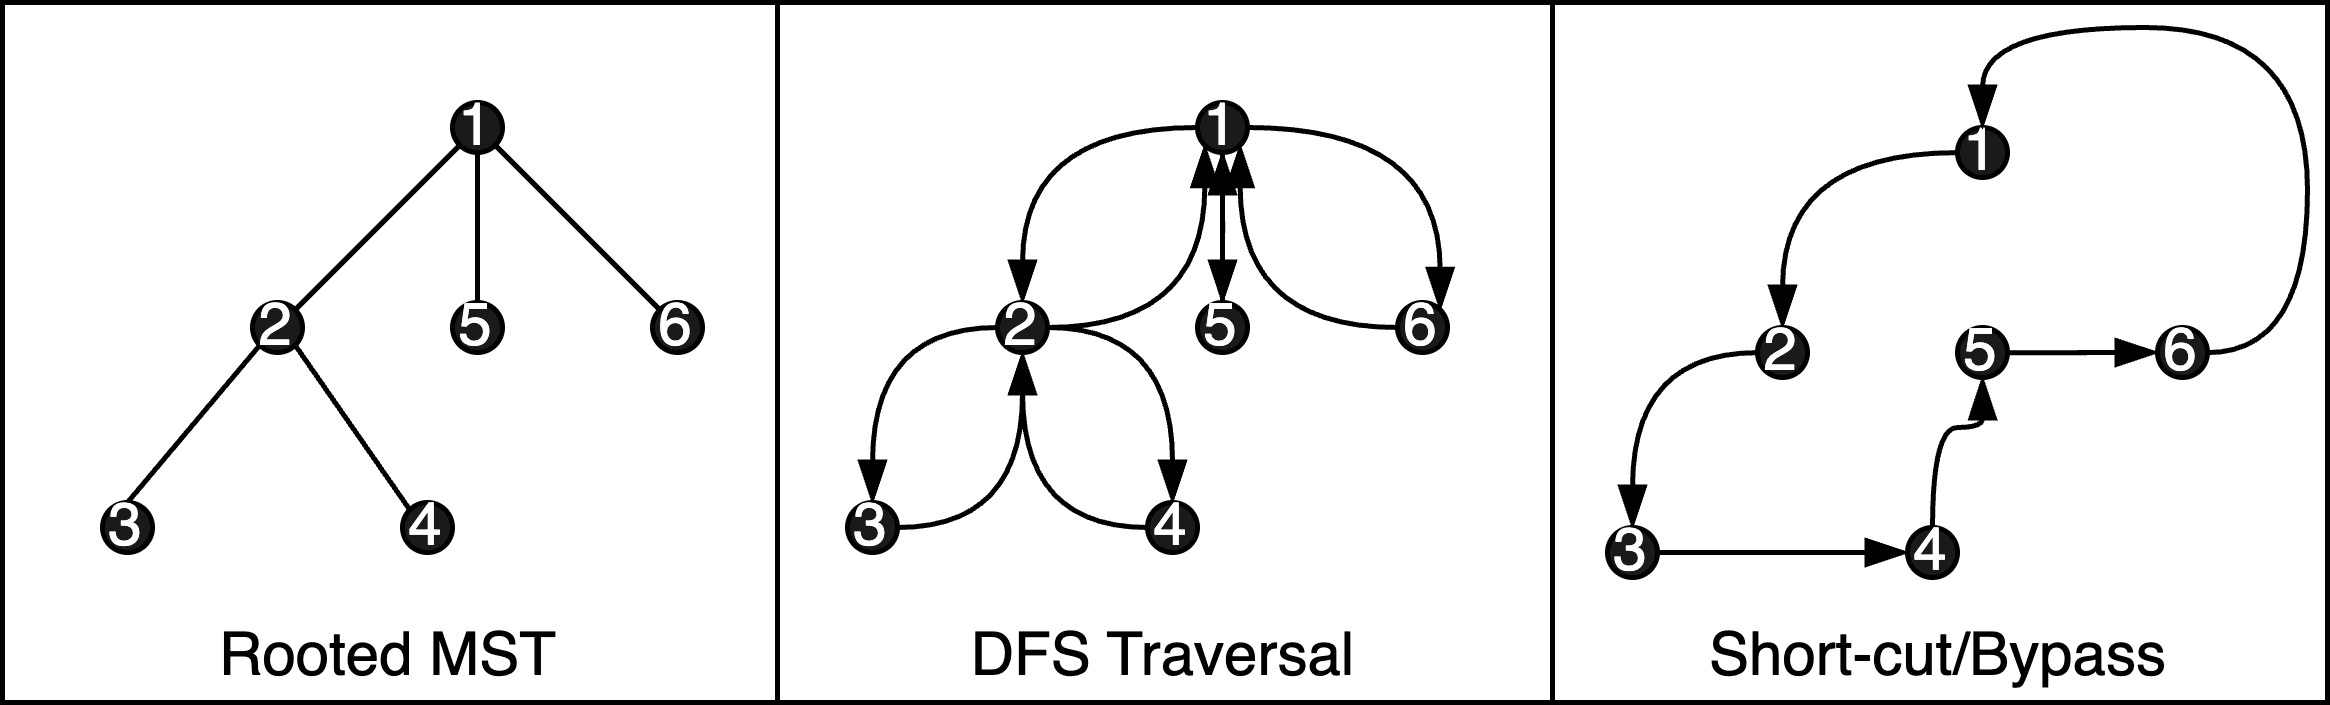
\includegraphics[width=0.9\linewidth]{../assets-v1/images/mst-2.png}
    \caption{近似比为2的算法(步骤)}
\end{figure}

证明如下:
\begin{itemize}
    \item 由e、三角形三条边关系定则,$c\left(C^\prime\right)\le c\left(C\right)$;
    \item 由c,$c\left(H_G^\ast\right)\geq c\left(H_G^\ast-e\right)\geq c\left(T\right)$;
    \item 由d,$c\left(C\right)=2\times c\left(T\right)$;
    \item 故$c\left(C^\prime\right)\le2c\left(H_G^\ast\right)$;
    \item 因此,该近似算法所得解,最多也不会超过最优解的2倍。
\end{itemize}

然后仍基于最小生成树,设法减小“每边下探一次,回溯一次”带来的额外开销,导出理论近似比为1.5的算法。
期待一笔画、不重边地遍历所有顶点,可以将问题转换成“欧拉回路”问题。无向图存在欧拉回路的充要条件为:该图为连通图,且所有顶点度数均为偶数。
倘若`奇度数`顶点为偶数个(证明见下),那么可以通过将其两两匹配,为每一个顶点都“附赠”一个度,这样便可以满足“顶点度数均为偶数”条件。

\begin{enumerate}[label= (\alph*)]
    \item 定义:$S$代表一系列边(允许重边),$c\left(S\right)$代表各边权重(长度)之和。
    \item 定义:$H_G^\ast$为无向多重图$G$上,长度最短的哈密尔顿回路(Hamiltonian Cycle),即途中经过所有点且只经过一次。
    \item 定义:假设$S$为无向多重图$G$上的导出子图,在$S$上长度最短的哈密尔顿回路记为$H_S^\ast$。根据三角形三边关系定则易证,$c\left(H_S^\ast\right)\le c\left(H_G^\ast\right)$。
    \item 构造最小生成树$T$,根据最小权生成树定义,$c\left(H_G^\ast\right)\geq c\left(H_G^\ast-e\right)\geq c\left(T\right)$。
    \item 分离在$T$上度数为奇数的点,生成导出子图$S$(根据握手定理,给定无向图$G=\left(V,E\right)$,一条边贡献2度,故有$\Sigma degG\left(v\right)=2\left|E\right|$;除开度数为偶数的顶点所贡献的度数,推论可知,度数为奇数顶点数有偶数个);
    \item 构造$S$的最小权完美匹配$M$,构造多重图$G^\prime=T\ \cup M$(此时每个顶点均为偶数度,故存在欧拉回路);
    \item 生成$G^\prime$的欧拉回路$C$,$c\left(C\right)=c\left(T\right)+c\left(M\right)$;
    \item 搭桥(short-cut/bypass)略过重复访问的点(起点终点不删)得到符合问题描述的新回路$C^\prime$(最后回到起点)。
\end{enumerate}

证明:
\begin{itemize}
    \item 由e、三角形三边关系定则,$c\left(C^\prime\right)\le c\left(C\right)$;
    \item 由d,$c\left(H_G^\ast\right)\geq c\left(H_G^\ast-e\right)\geq c\left(T\right)$;
    \item 由g,$c\left(C\right)=c\left(T\right)+c\left(M\right)$;
    \item 由f、c,$c\left(M\right)+c\left(M\right)\le c\left(M1\right)+c\left(M2\right)=c\left(H_S^\ast\right)\le c\left(H_G^\ast\right)$;
    \item 故$c\left(C^\prime\right)\le c\left(T\right)+c\left(M\right)\le c\left(H_G^\ast\right)+\frac{1}{2}c\left(H_G^\ast\right)$;
    \item 即得证。
\end{itemize}

\begin{figure}[htbp]
    \centering
    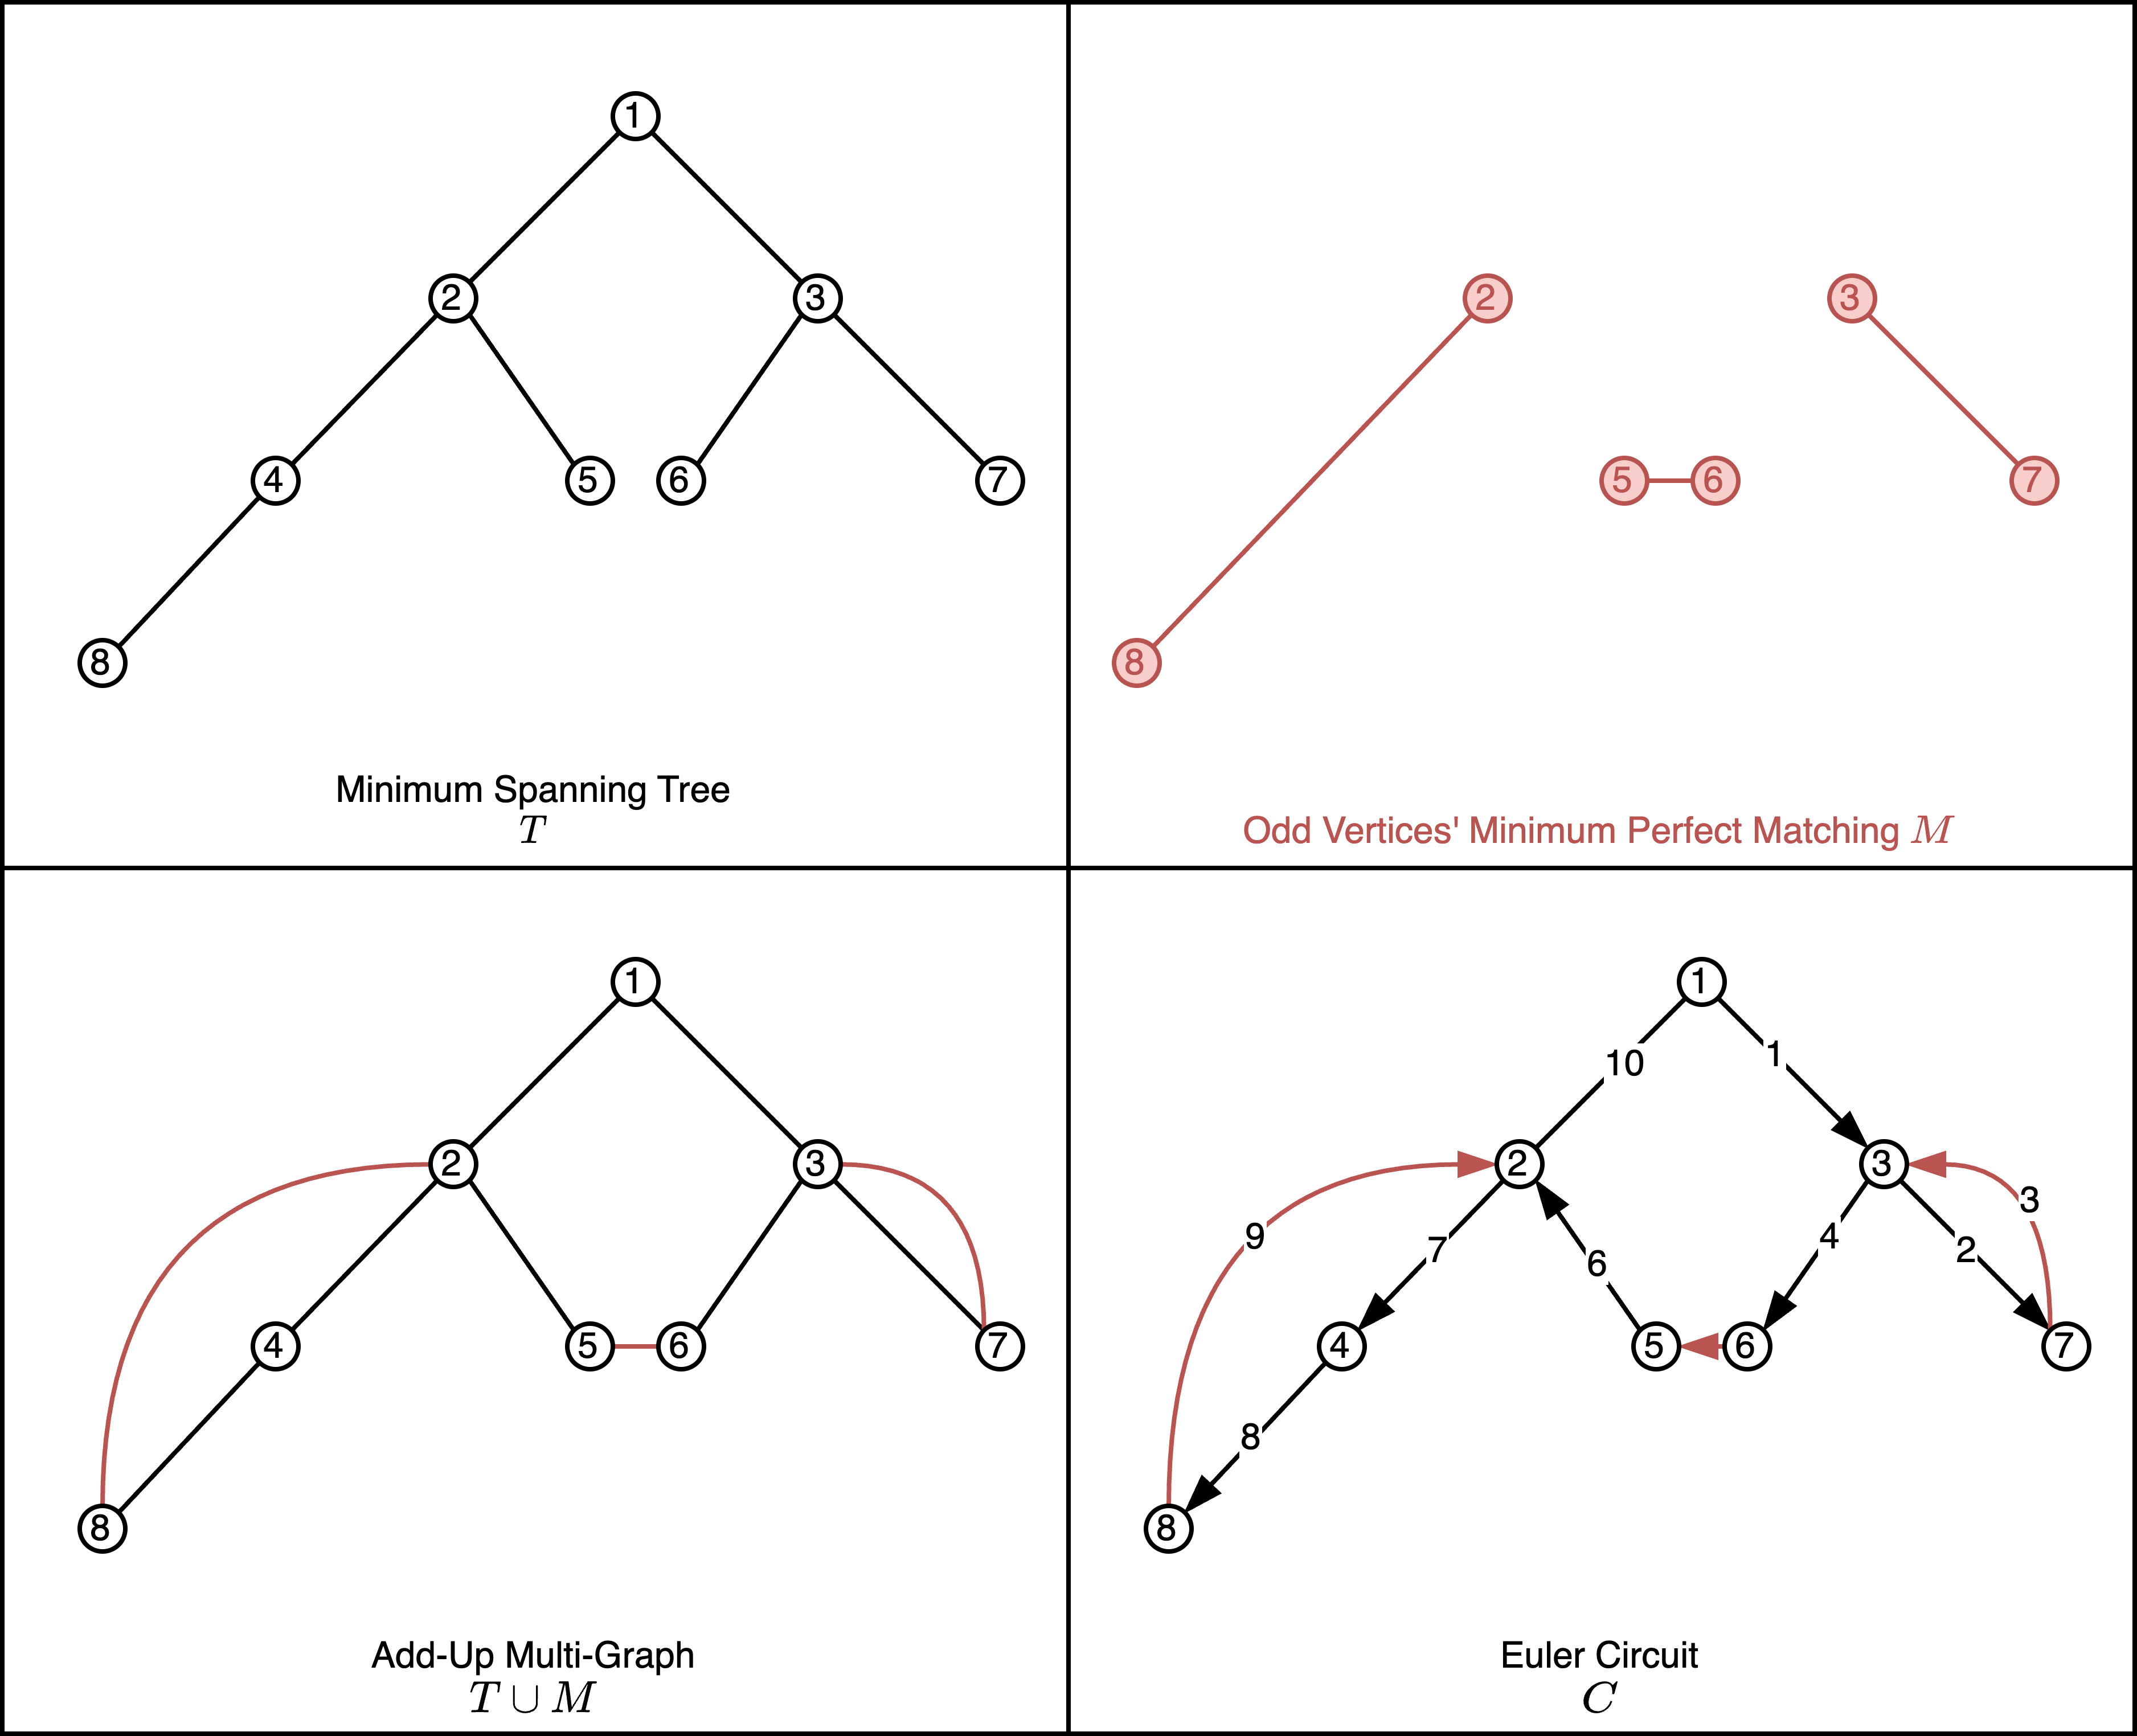
\includegraphics[width=0.72\linewidth]{../assets-v1/images/Euler.png}
    \caption{克里斯托菲德斯算法(步骤)}
\end{figure}

\begin{figure}[htbp]
    \centering
    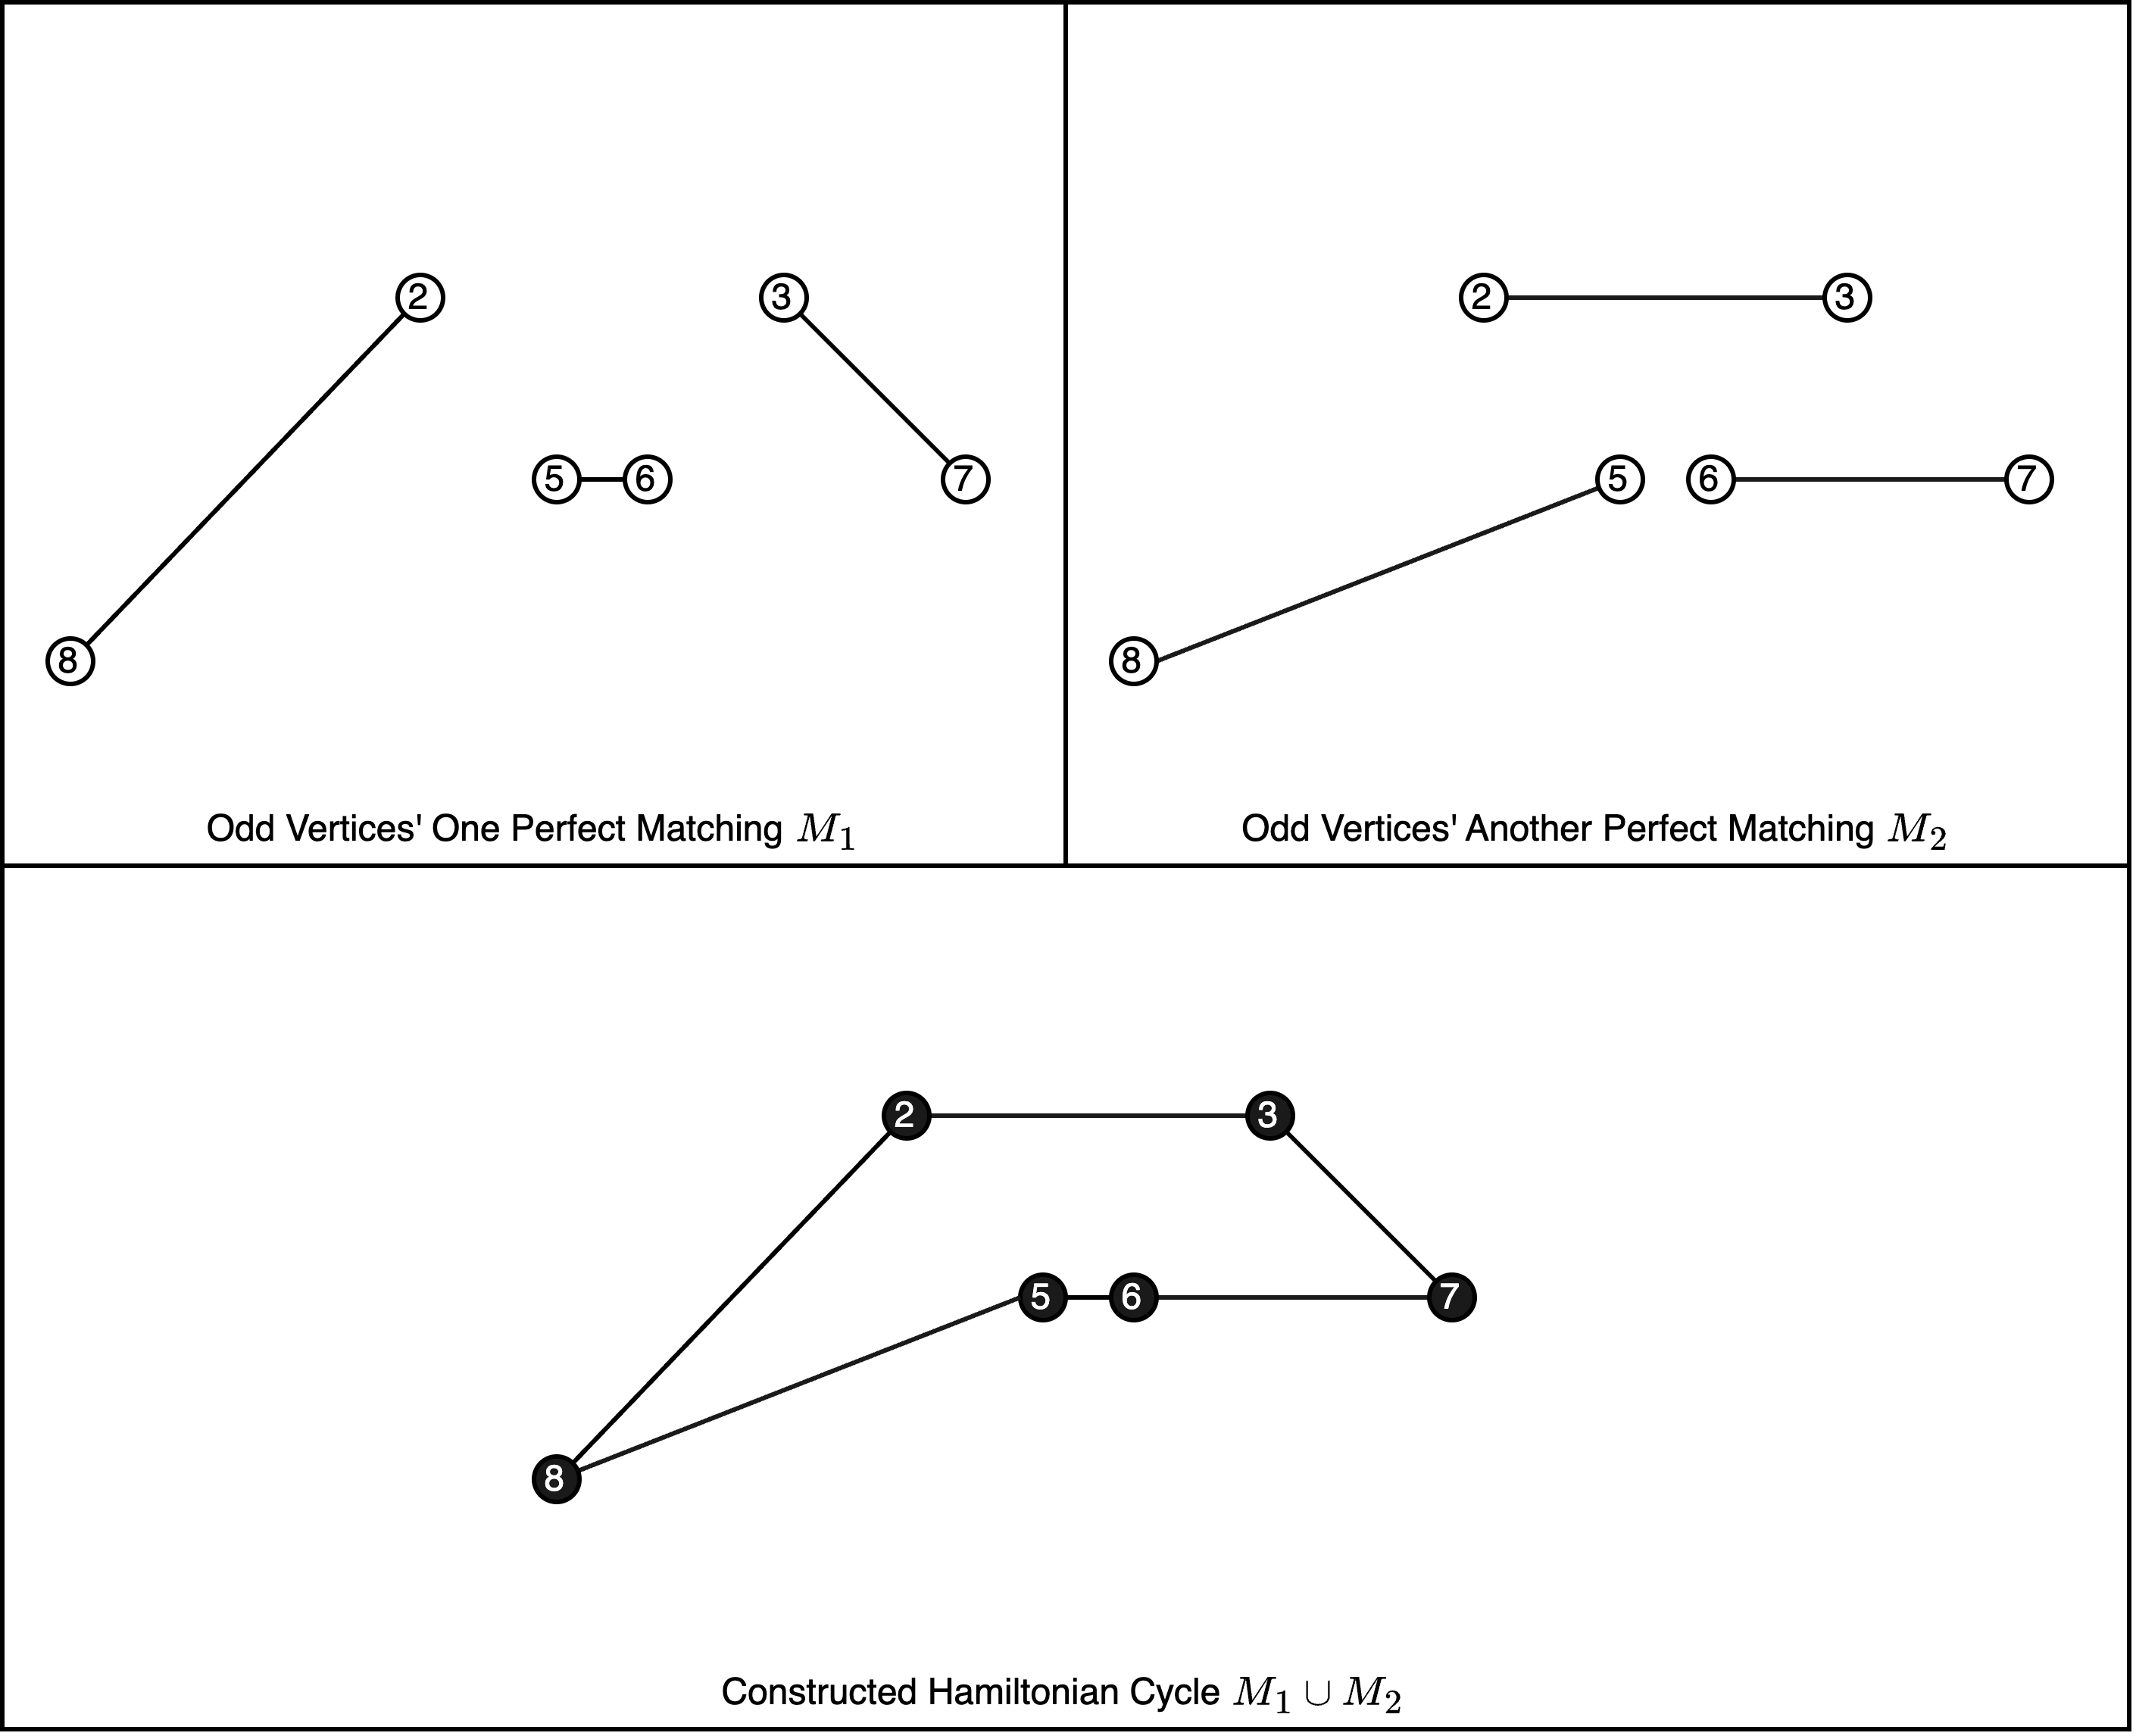
\includegraphics[width=0.72\linewidth]{../assets-v1/images/match.png}
    \caption{最小权完美匹配(举例)}
\end{figure}

\begin{figure}[htbp]
    \centering
    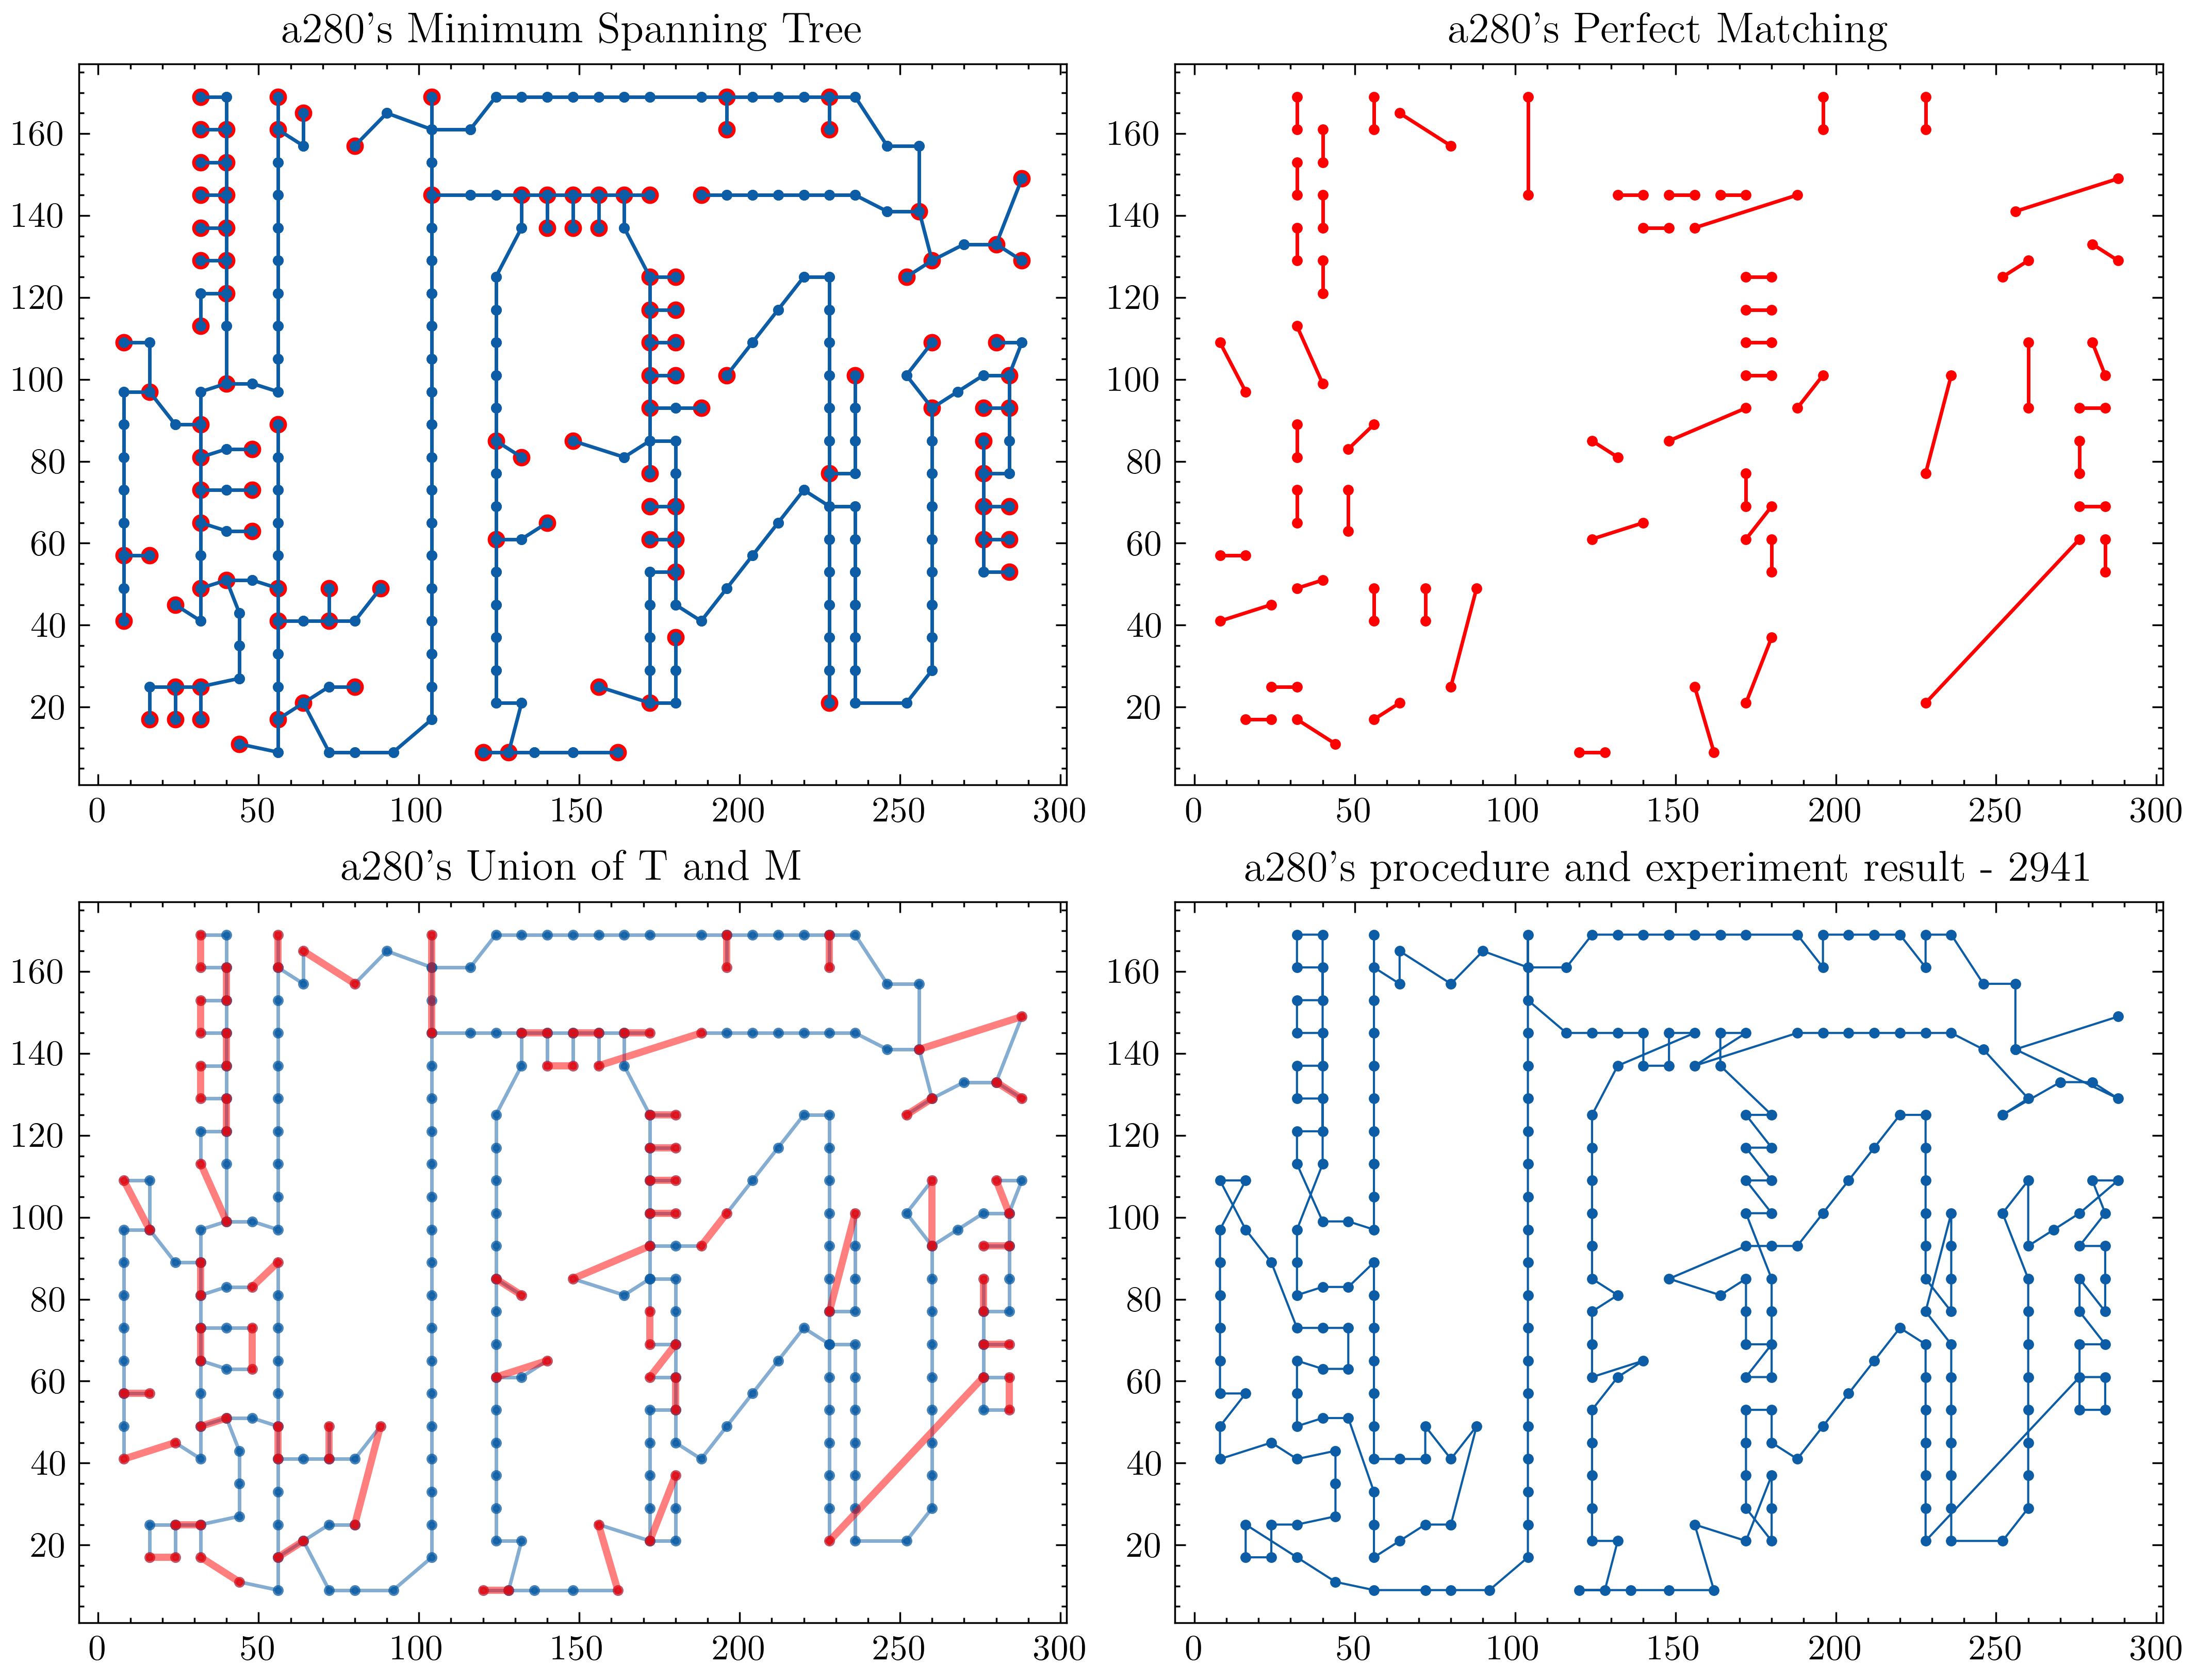
\includegraphics[width=0.7\linewidth]{../assets-v1/illustrations/christofides - a280's procedure and experiment result - 2941.png}
    \caption{克里斯托菲德斯算法(实例)}
\end{figure}

\subsubsection{2-OPT改进算法}

“如果题目数据使用欧几里得距离,那么最优路线必定不会自交”。
基于这一观察,有学者倡导使用“改进”算法,即对于一条可行回路查漏补缺对其进行细微调整。

“知错能改,善莫大焉”。“怎么改”对应着一种“邻域操作”(函数、变换、系统、算子)。

解空间中的一个巡回旅行路线直接或间接对应一个全排列$\sigma$,若将其视作$n$维空间中的一个点,其邻域$\sigma^\prime$操作有很多种,如插入、块插入、块反转、点对换、块交换、边重组等等。
边重组中,最著名的是2-交换(2-OPT)、3-交换(3-OPT)。2-交换的步骤就是删除路线中的两条边,用另外两条更短的边重新连接,使路径再次连为一体。反复使用2-交换算子改进路线,可以在很大程度上改进“虎头蛇尾”、“目光短浅”的回路路线。
\begin{figure}[htbp]
    \centering
    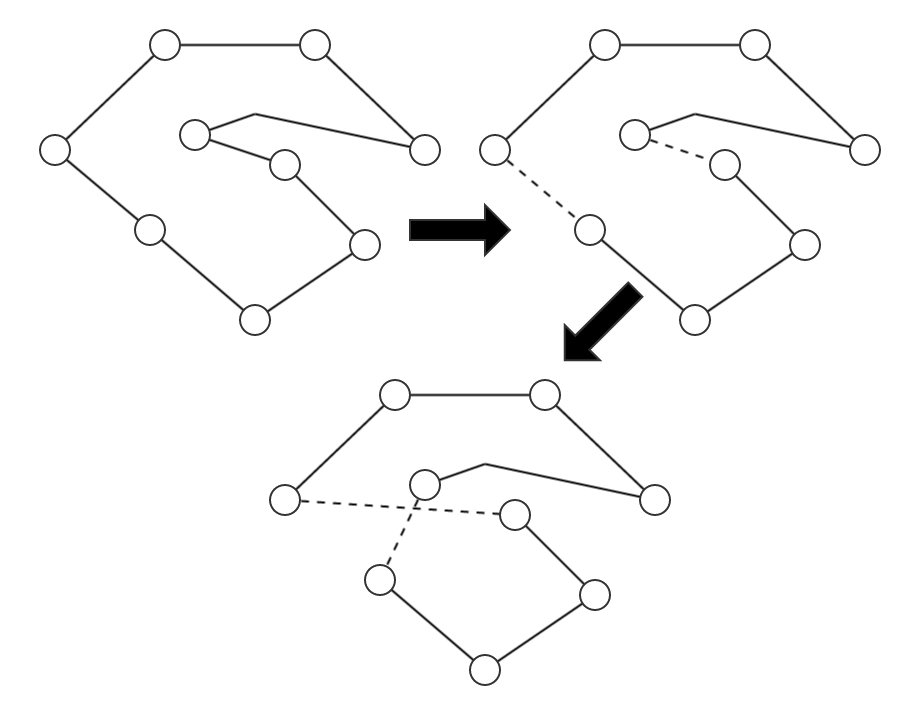
\includegraphics[width=0.35\linewidth]{../assets-v1/images/opt-2.png}
    \caption{2-OPT(图例)}
\end{figure}

2-OPT改进算法伪代码如下:

\IncMargin{1em}
\begin{algorithm}[H]
    \SetKwInOut{Input}{input}\SetKwInOut{Output}{output}

    \Input{$V=\{v_1, \ldots, v_n\}, dist(\cdot, \cdot), L(\cdot), \sigma$}
    \Output{$\sigma^*$}
    \BlankLine
    $length \leftarrow L(\sigma)$\;
    \Repeat{$\neg improved$}{
        $improved \leftarrow \text{False}$\;
        \For{$i \leftarrow 0$ \KwTo$n-3$}{
            \For{$j \leftarrow i+2$ \KwTo$n$}{
                $\sigma^\prime \leftarrow \sigma$\;
                $\sigma^\prime[i+1 \ldots j] \leftarrow \text{reverse}(tour^\prime[i+1 \ldots j])$\;
                $length^\prime \leftarrow L(\sigma^\prime)$\;
                \If{$length^\prime < length$}{
                    $\sigma \leftarrow \sigma^\prime$\;
                    $length \leftarrow length^\prime$\;
                    $improved \leftarrow \text{True}$\;
                }
            }
        }
    }
    $\sigma^* \leftarrow \sigma$\;
    \caption{2-OPT Algorithm}
\end{algorithm}
\DecMargin{1em}

3-OPT改进算法与之类似,但是可能的情况更多:
\begin{figure}[htbp]
    \centering
    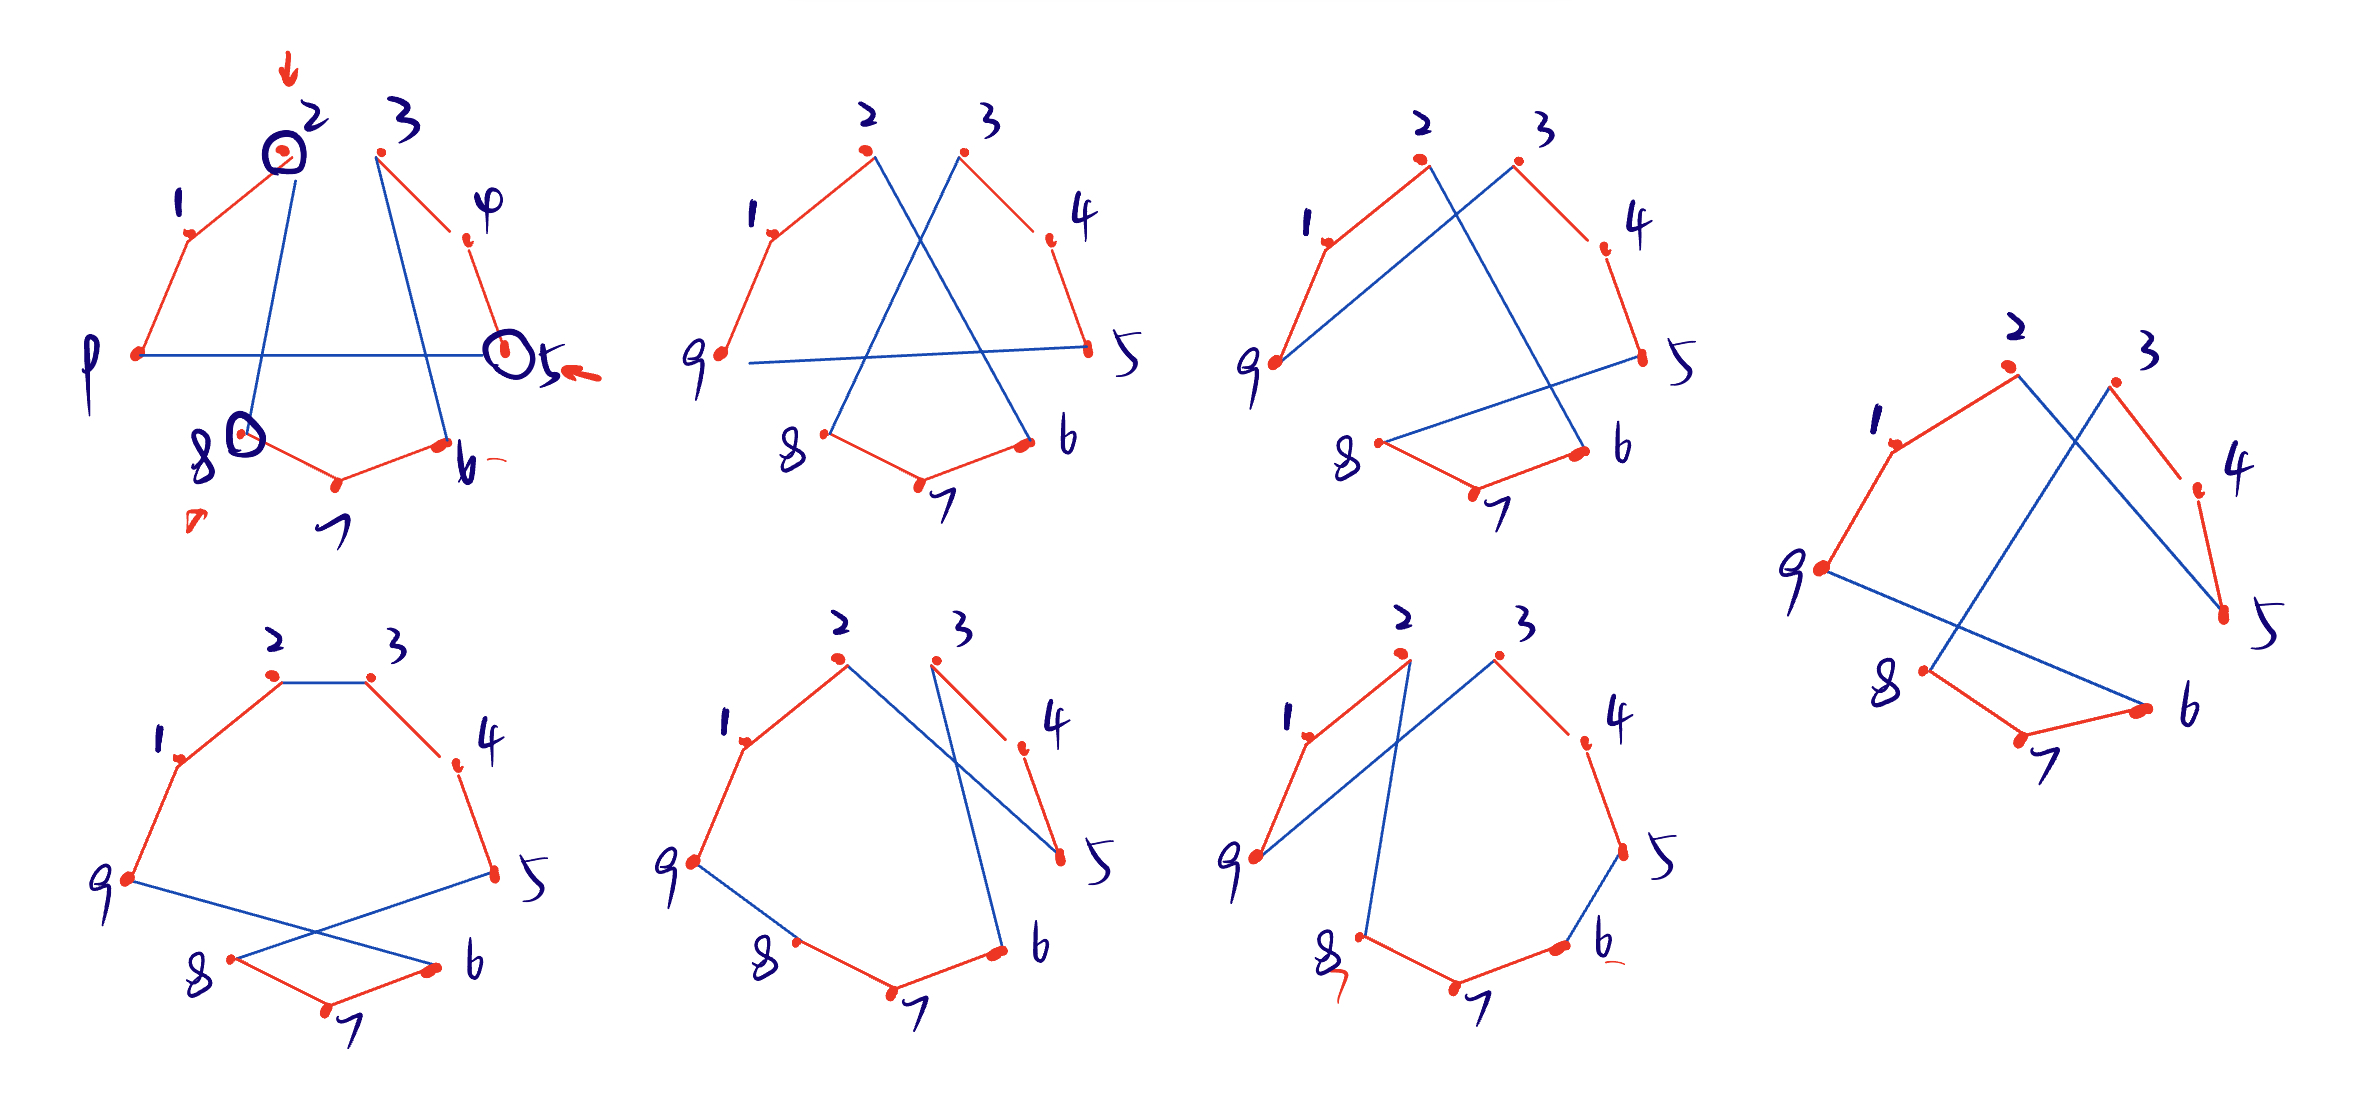
\includegraphics[width=1.0\linewidth]{3-opt.jpeg}
    \caption{3-OPT(图例)}
\end{figure}

\subsection{随机型近似算法}

\subsubsection{王磊算法}

王磊老师在课上跟学生说过一个随机型近似算法(王磊算法),基本算法$A_1$描述如下:

\textbf{输入:} 指导序列$\gamma$,$\gamma$是所有顶点的一个全排列;

\textbf{开局:} 用$\gamma$前$3$个点绘制外接凸多边形(三角形),构成初始回路$\sigma = (\gamma(1), \gamma(2), \gamma(3))$;

\textbf{迭代:} 每次从当前格局向新格局演化时,取出下一个点,按照使得新的部分回路长度尽量短的贪心策略,将其插入至$\sigma$合适的位置;

\textbf{停机:} 直至产生$n$个点的回路$\sigma$,算法结束,输出$\sigma$。

\IncMargin{1em}
\begin{algorithm}[H]
    \SetKwInOut{Input}{input}\SetKwInOut{Output}{output}
    \Input{$V=\{v_1, \ldots, v_n\}, dist(\cdot, \cdot), \gamma$ a permutation of $V$}
    \Output{$\sigma$ the tour}
    \BlankLine
    $\sigma \leftarrow (\gamma(1), \gamma(2), \gamma(3))$\;
    \For{$i \leftarrow 4$ \KwTo $n$}{
        $best\_idx \leftarrow \argmin\limits_{j \in \{1, \ldots, |\sigma|\}}  L(\sigma_{1:j}) + dist(\gamma(i), \sigma(j)) + L(\sigma_{j:|\sigma|}) - L(\sigma) $\;
        $\sigma \leftarrow (\sigma_{1:best\_idx}, \gamma(i), \sigma_{best\_idx+1:|\sigma|})$\;
    }
    \caption{Generate Tour from a Conductor}
\end{algorithm}
\DecMargin{1em}

对所有指导序列$\gamma \in \Gamma$,目标是$\gamma^\star = \argmin\limits_{\gamma \in \Gamma} L(A_1(\gamma))$。据此,王磊又提出算法$A_2$:

\textbf{初始格局:} 初始化$\gamma$,通过$A_1$算法指导获得回路$\sigma = A_1(\gamma)$,以及长度$l = L(\sigma)$;

\textbf{邻域搜索:} 邻域变换得到$\gamma^\prime$、$\sigma^\prime$及$l^\prime$,若$l^\prime < l$,依照最陡下降法,更新格局$\gamma \leftarrow \gamma^\prime$

\textbf{跳坑策略:} 当$\gamma$位于局部最优,即几乎尝试所有邻域都无法改善目标函数时,重新随机初始化$\gamma$或者采用大步长算子(如块移动、块对换、块插入)对$\gamma$进行变换。

\begin{algorithm}[H]
    \SetKwInOut{Input}{input}\SetKwInOut{Output}{output}
    \Input{$V, dist(\cdot, \cdot), L(\cdot), epoch, early\_stop$ \\
        $permutation(\cdot), transform(\cdot), shuffle(\cdot)$}
    \Output{$\sigma, l$}
    \BlankLine
    $\gamma \leftarrow permutation(V)$; $\sigma \leftarrow A_1(\gamma)$; $l \leftarrow L(\sigma)$\;
    \For{$e \leftarrow 1$ \KwTo $\text{epoch}$}{
        $\gamma^\prime \leftarrow transform(\gamma)$; $\sigma^\prime \leftarrow A_1(\gamma^\prime)$; $l^\prime \leftarrow L(\sigma^\prime)$\;
        \If{$l^\prime < l$}{
            $\gamma \leftarrow \gamma^\prime$; $\sigma \leftarrow \sigma^\prime$; $l \leftarrow l^\prime$\;
        }
        \If{no improvement for \text{early\_stop} iterations}{
            $\gamma \leftarrow permutation(V)$ or $\gamma \leftarrow shuffle(\gamma)$\;
        }
    }
    % $\sigma^* \leftarrow \sigma$; $l^* \leftarrow l$\;
    \caption{WangLei Algorithm}
\end{algorithm}

王磊算法的创新和启发意义主要有以下三点:

\begin{enumerate}
    \item 传统启发算法求解旅行商问题,几乎全部都是直接在回路$\sigma$上进行邻域扰动,获得新解。而王磊算法则提出了$\gamma \to \sigma$的映射算法$A_1$,这相当于对原有解空间进行了“扭曲”,将求“回路”的原问题转化为了求“指导顺序“的新问题。

          最优化理论中,原始问题很难求解时,往往通过引入对偶问题的方式,简化对原始问题的求解。在机器学习中,也有代替函数、核函数作为例子。但是,我们不禁要问,对于所有的“指导序列”$\gamma \in \Gamma$,它们所生成的所有回路集合$\Sigma^\star$,是否包含了最优回路$\sigma^\star$?

          即,通过指导序列将问题转换,问题转换前后是否仍然具有“一致性”  ?

    \item 邻域搜索和跳坑策略思想并不高深。局部极小值的定义来自于函数求极值,跳坑则更有烟火气:如果你已经期末总评满分了,就要跳坑,到更有希望的学府继续深造。

          无论是回路$\sigma$还是指导序列$\gamma$都是高维空间的一个点,若其邻域中的“点”所对应的回路长度都不比中心点短,则该中心点是局部极小值点;当邻域搜索陷入局部极小值点时,就应该采用“跳坑策略”,进行随机扰动,跳出陷阱,继续邻域搜索。

          这其中的问题有二:一是“随机扰动”算子和所谓“邻域算子”在本质上究竟有何不同?设计的“邻域算子”真的在逻辑上只是轻微的扰动吗?二是随着邻域算子设计的不同,邻域中的“点”随着维度的增大,个数可能比想象中要多得多,因此有时候又不得不采用固定次数的方式来执行邻域搜索,导致邻域开采不足。邻域搜索对应“变异”、“开采”,而跳坑策略则对应“探索”,可以说所有的最优化算法都要考虑这两者的平衡。

    \item 生成回路算法本身也具有烟火气。想象一下,借一个扎头发的橡皮筋,套住几个点;然后采用贪心策略,将其余点加入回路。

          传统的最近邻点贪心策略是,最后一步方能连成回路,这就导致目光浅显、虎猴蛇尾;而如果是在一个成形的“回路”中添加,每次添加评价的都直接是回路的全长,则能一定程度上缓解“短视”问题。
          这启发我们同样是贪心策略,但是如何运用,运用的好不好是可以评价的,是有优劣的。
\end{enumerate}

\subsubsection{模拟退火}

事实上,人们从物理世界状态演化、自然界各种现象、千百年来生存斗争经验获得启发,以仿生拟人拟物途径设计了各种算法。模拟退火是一种,具有自然背景且实现简单。

模拟退火并没有显式地将跳坑策略(探索)和邻域搜索(开采)分成两阶段看待;它的基本思想是,以概率接受劣解,且接受劣解的概率随迭代次数递减直至无限趋近于零。
如果只接受优解,则容易早熟,多样性不足,易于陷入局部最优,因此需要接受劣解;
如果一味接受劣解,则无法保证收敛性,因此需要控制接受劣解的概率;模拟退火算法中,
随着迭代次数递增,温度越低,对劣解的容忍程度越低,可以保证算法不至于震荡,可以收敛。

\IncMargin{1em}
\begin{algorithm}[H]
    \SetKwInOut{Input}{input}\SetKwInOut{Output}{output}
    \Input{$V, dist(\cdot, \cdot), L(\cdot),transform(\cdot)$\\
        $T, \epsilon, \alpha, time\_out, early\_stop$}
    \Output{$\sigma^*, L^*$}
    \BlankLine
    $\text{start\_time} \leftarrow \text{current time}$\;
    \While{$\text{current time} - \text{start\_time} < time\_out$}{
        $\sigma \leftarrow \text{permutation}(V)$\;
        $L \leftarrow L(\sigma)$\;
        \While{$T > \epsilon$}{
            \For{$step \leftarrow 1$ \KwTo $early\_stop$}{
                $\sigma^\prime \leftarrow \text{transform}(\sigma)$; $L^\prime \leftarrow L(\sigma^\prime)$; $\Delta L \leftarrow L^\prime - L$\;
                \If{$\Delta L < 0$ \textbf{or} $\text{random}(0,1) \leq e^{\frac{-\Delta L}{T}}$}{
                    $\sigma \leftarrow \sigma^\prime$; $L \leftarrow L^\prime$\;
                }
            }
            $T \leftarrow T \times \alpha$\;
        }
    }
    $\sigma^* \leftarrow \sigma$, $L^* \leftarrow L$\;
    \caption{SimulatedAnnealing Algorithm}
\end{algorithm}
\DecMargin{1em}

\section{遗传算法及改进策略}

\subsection{传统的遗传算法}

% 遗传算法的框架伪码如下:

\IncMargin{1em}
\begin{algorithm}[H]
    \SetKwInOut{Input}{input}\SetKwInOut{Output}{output}
    \Input{$V, \text{epoch}, \text{early\_stop}, \text{population\_size}, \text{pc}, \text{pm}$}
    \Output{$\sigma^*, L^*$}
    \BlankLine
    初始化种群\;
    \For{$e \leftarrow 1$ \KwTo $\text{epoch}$}{
        初始化当前最佳长度为无穷大\;
        \For{$step \leftarrow 1$ \KwTo $\text{early\_stop}$}{
            选择操作:根据适应度选择当前种群中的一些个体\;
            交叉操作:根据交叉概率 $\text{pc}$ 结合选中的个体产生后代\;
            变异操作:根据变异概率 $\text{pm}$ 改变某些个体的特征\;

            如果找到更优的解,则更新当前最佳长度\;
        }
        重新初始化种群\;
    }
    $\sigma^* \leftarrow$ 找到的最佳解; $L^* \leftarrow$ 最佳解的长度\;
    \caption{Genetic Algorithm for TSP}
\end{algorithm}
\DecMargin{1em}

无论是基于邻域搜索和拟人策略跳坑的王磊算法,
还是从淬火物理结晶过程获得启发的模拟退火算法,
都是基于“个体”的启发算法。
而遗传算法,从生物学获得启发,将“个体”扩展至“种群”;
除邻域操作(也成“变异”算子)外,新增了“交叉”操作,
将“个体理性”和“群体理性”进行结合。传统的遗传算法求解旅行商问题的具体细节为:

\begin{description}
    \item[编码] 将执行变异操作的个体直接编码为城市序号的全排列$\sigma$;
    \item[适应] 采用$\frac{1}{L(\sigma)}$表示解的优劣,适应度越大,被选择保留的概率越高;
    \item[选择] 采用轮盘赌,计算每条染色体的被选择概率和累计概率,再根据一个随机数确定要保留的染色体;选择操作是遗传算法的核心,一方面,要保证收敛质量好,即回路长度短,另一方面,要保证种群有足够的多样性,避免陷入局部最优的困境;
    \item[交叉] 交叉操作的目的是,集合不同回路的优良回路特征,常用有顺序交叉和部分映射交叉。
    \item[变异] 通过邻域变换对种群中的个体(回路)进行扰动;遗传算法中,变异概率通常非常小。
\end{description}

\subsection{改进的遗传算法}

在编码部分,仍采用整数回路直接编码;在交叉部分,沿用顺序交叉和部分映射交叉。

然后,对传统遗传算法的初始化、选择、变异操作做出如下改进,后文称为\textbf{GIGA}:
\begin{description}
    \item[初始] 发扬“继承”策略,在初始化阶段,将“2-OPT”和“最近邻点”算法的结果回路作为初始化种群的一部分;这样可以极大的减少迭代次数,在交叉过程中吸取各个算法最优解的优良局部特征,而且保证了解的收敛性,使得其回路长度最大不会超过最优回路的1.5倍,最差仍有理论保证兜底。其实,这变相地把“遗传算法”视作一种“群智融合”和“回路改进”方法,通过融合、修补、改进已有的解来使目标值更理想。
    \item[选择] 在选择过程中,弃用轮盘赌法。轮盘赌法的缺陷是,当适应度相似时,选择概率值相近,不一定保证选择当前种群中回路长度最小的个体,这使得算法收敛困难;改用排位等级法,以回路长度从小到达排序,以排序等级确定选择概率,缓解了适应度相近时选择困难的问题。
    \item[变异] 在变异过程中,除了使用传统的算子外(点插入、块插入、块反转、点对换、块对换、2-OPT、3-OPT),我从王磊$A_1$算法中获得启发,设计了一个全新的变异算子:贪婪插入。采用“最陡下降法”,我们对于一个已知回路$\sigma$,随机剔除$N$个城市,然后依序采取贪心策略将被剔除的点添加到回路中。$N$取自一个概率分布,这样能够保证剔除城市个数可以动态变化;而剔除策略,可以分为单点剔除和随机剔除。
\end{description}

\newpage
下面给出种群初始化的伪代码:

\IncMargin{1em}
\begin{algorithm}[H]
    \SetKwInOut{Input}{input}\SetKwInOut{Output}{output}
    \Input{$V$, $size$, $init\_population$}
    \Output{Initialized population $P$}
    \BlankLine
    $P \leftarrow init\_population$\;
    \While{$|P| < size$}{
        $P$.append(permutation($V$))\;
    }
    \caption{Population Initialization for Genetic Algorithm}
\end{algorithm}
\DecMargin{1em}

下面给出选择操作的伪代码:

\IncMargin{1em}
\begin{algorithm}[H]
    \SetKwFunction{Select}{Select}
    \SetKwProg{Fn}{Function}{:}{}
    \Fn{\Select{$P, L, size, C, operator$}}{
        $lengths \leftarrow [L(individual) \text{ for each } individual \in P]$\;
        $order \leftarrow$ sort indices of $lengths$ in ascending order\;
        $selected \leftarrow [\text{best seen tour}]$\;
        \While{$|selected| < size$}{
            $idx \leftarrow 0$, $target \leftarrow 1$\;
            \While{$\text{random}(0,1) < target \times (1 - C)$}{
                $idx \leftarrow idx + 1$\;
                $target \leftarrow target \times C$\;
            }
            $selected$.append($P[order[idx]]$)\;
        }
        \KwRet{$selected$}\;
    }
    \caption{Selection Operation in Genetic Algorithm}
\end{algorithm}
\DecMargin{1em}

下面给出变异算子的伪代码:

\IncMargin{1em}
\begin{algorithm}[H]
    \SetKwInOut{Input}{input}\SetKwInOut{Output}{output}
    \Input{$\sigma$, $dist(\cdot, \cdot)$, $times$, $dimension$}
    \Output{Modified $\sigma$}
    \BlankLine
    \eIf{$\text{random}(0,1) < 0.5$}{
        $conductor \leftarrow$ remove $times$ random elements from $\sigma$\;
    }{
        $pivot \leftarrow \text{random integer}(1, dimension - times - 1)$\;
        $conductor \leftarrow$ remove $times$ elements starting at $pivot$ from $\sigma$\;
    }
    \ForEach{$vertex \in conductor$}{
        $best\_idx \leftarrow \argmin\limits_{j \in \{1, \ldots, |\sigma|\}}  L(\sigma_{1:j}) + dist(vertex, \sigma(j)) + L(\sigma_{j:|\sigma|}) - L(\sigma) $\;
        $\sigma \leftarrow (\sigma_{1:best\_idx}, vertex, \sigma_{best\_idx+1:|\sigma|})$\;
    }
    \caption{Greedy Insert Operator for Genetic Algorithm}
\end{algorithm}
\DecMargin{1em}

\section{实验设置与测试结果}

\subsection{数据集与超参数设置}

TSPLIB(\url{http://comopt.ifi.uni-heidelberg.de/software/TSPLIB95/})中公布了旅行商问题的benchmark测试数据集。
以EUC-2D类型的测试数据集中的实例a280为例,
a280.txt文件开头有一段说明文字,然后是280(表示点的个数),接下来有280行数据,每行数据含有3个数,分别是:当前点的序号、当前点的x坐标、当前点的y坐标。

\begin{table}[htbp]
    \caption{随机近似算法实验超参数设置}
    \centering

    \begin{threeparttable}
        \begin{tabular}{rll}
            \toprule
            对应算法                  & 超参数                                   & 缺省值                    \\
            \midrule
            GreedyNearestNeighbor & $boost$, 是否随机选择一个起始城市                 & $True$                 \\
            SimulatedAnnealing    & 初始温度$t$, 终止温度$\epsilon$, 衰减系数$\alpha$ & $1000, 10^{-14}, 0.98$ \\
            SimulatedAnnealing    & 重启停机参数time\_out, early\_stop          & $1, 250$               \\
            WangLeiAlgorithm      & 重启停机参数epoch, early\_stop              & $16, 250$              \\
            Proposed GIGA         & 种群大小$size$, 交叉概率$p_c$,变异概率$p_m$       & $50, 1, 0.4$           \\
            Proposed GIGA         & 选择系数$C$                               & $0.5$                  \\
            Proposed GIGA         & 重启停机参数epoch, early\_stop              & $6, 7500$              \\
            \bottomrule
        \end{tabular}
        \zihao{-5}
        \begin{tablenotes}
            \item [*]   提出改进的遗传算法的初始种群仅来自2-OPT、GreedyNearestNeighbor。
        \end{tablenotes}
    \end{threeparttable}
    \qquad
\end{table}

\subsection{实验结果}
王磊老师在VC6.0开发环境中将算法用C语言编程,在CPU主频为3.4GHz的微机上进行的测试;
我在是在macOS 13.5.2 (22G91)系统下以Python~3.9.12进行编程。

由于编程语言、环境的巨大差异,运算结果无法相互比较。因此,我弃用了《专业方向综合实践验收的问题》的报道结果,
自行复现了王磊算法作为对比算法进行测试、对比。

代码开源在:\url{https://github.com/DURUII/Homework-Algorithm-TSPLIB95}。

选取城市数小于等于1000中全部48个benchmark测试用例进行测试,两点间距离四舍五入取整,每个实例计算10次。
下面是改进的遗传算法、王磊算法、模拟退火算法计算10次,所得回路长度的最小值$L_{\min}$、平均值$L_{\text{avg}}$和平均计算时间$t_{\text{avg}}$。

本文提出的改进的遗传算法,在\textbf{1}个测试用例中超过王磊算法或已求得最优解;在剩余\textbf{}个测试用例中,平均回路长度不超过王磊算法的\textbf{\%},最短回路长度不超过王磊算法的\textbf{\%}。
所有测试用例中,算法所给出的最小回路长度,与最优回路相比,平均最小相对误差为\textbf{0.73\%},低于\textbf{1\%}。
以a280这个benchmark为例,最优解的回路长度是\textbf{2579},算法所求最小长度为\textbf{2584},算法所给出的最小回路长度相对误差为\textbf{0.19\%}。

\newpage
\begin{table}[htbp]
    % \caption{算法运行统计结果}
    \scriptsize
    \centering
    \begin{tabular}{rcccccccccc}
        \toprule
        \multicolumn{2}{c}{Benchmark} & \multicolumn{3}{c}{Proposed GIGA} & \multicolumn{3}{c}{WangLei} & \multicolumn{3}{c}{SimulatedAnnealing}                                                                                                                                                  \\
        \cmidrule(l){1-2} \cmidrule(l){3-5} \cmidrule(l){6-8} \cmidrule(l){9-11}
        Name                          & $L_{\text{OPT}}$                  & $L_{\min}$                  & $L_{\text{avg}}$                       & $t_{\text{avg}}$ & $L_{\min}$              & $L_{\text{avg}}$ & $t_{\text{avg}}$ & $L_{\min}$            & $L_{\text{avg}}$ & $t_{\text{avg}}$ \\
        \midrule
        a280                          & 2579                              & $\textbf{2584}^\dag$        & 2593.30                                & 312.50           & 2615                    & 2653.30          & 380.50           & 2792                  & 2890.40          & 43.76            \\
        berlin52                      & 7542                              & $\textbf{7542}^\star$       & 7542.00                                & 36.73            & $\textbf{7542}^\star$   & 7542.00          & 4.79             & $\textbf{7542}^\star$ & 7759.30          & 8.06             \\
        bier127                       & 118282                            & 120843                      & 121648.60                              & 97.18            & $\textbf{118326}^\dag$  & 119221.50        & 51.17            & 121173                & 124320.50        & 19.63            \\
        ch130                         & 6110                              & 6189                        & 6198.00                                & 93.35            & $\textbf{6115}^\dag$    & 6131.90          & 43.74            & 6355                  & 6548.00          & 19.89            \\
        ch150                         & 6528                              & 6588                        & 6588.00                                & 112.96           & $\textbf{6554}^\dag$    & 6582.50          & 65.98            & 6938                  & 7069.70          & 22.98            \\
        d198                          & 15780                             & 15831                       & 15888.30                               & 194.36           & $\textbf{15818}^\dag$   & 15860.00         & 141.29           & 16211                 & 16464.80         & 30.36            \\
        d493&35002& $\textbf{35544}^\dag$ &35560.27 &1239.37 &35670&35838.82 &3028.20 &39580&40399.09 &110.69 \\
        d657&48912& $\textbf{49852}^\dag$ &49900.80 &2429.40 &50101&50247.40 &7525.27 &61152&62870.10 &157.57 \\
        eil51                         & 426                               & 435                         & 435.40                                 & 254.25           & $\textbf{426}^\star$    & 427.00           & 31.93            & 429                   & 435.60           & 48.15            \\
        eil76                         & 538                               & 546                         & 546.00                                 & 374.14           & $\textbf{542}^\dag$     & 545.10           & 89.43            & 556                   & 560.20           & 75.42            \\
        eil101                        & 629                               & 639                         & 641.20                                 & 473.52           & $\textbf{633}^\dag$     & 636.30           & 162.24           & 656                   & 665.70           & 92.91            \\
        fl417&11861&11962&11977.00 &947.40 & $\textbf{11899}^\dag$ &11933.20 &1360.14 &13088&13604.10 &90.50 \\
        gil262                        & 2378                              & 2394                        & 2402.50                                & 459.81           & $\textbf{2391}^\dag$    & 2411.30          & 519.80           & 2541                  & 2628.20          & 71.41            \\
        kroA100                       & 21282                             & 21282                       & 21381.60                               & 570.70           & $\textbf{21282}^\star$  & 21286.00         & 215.12           & 21786                 & 22395.20         & 115.93           \\
        kroB100                       & 22141                             & 22364                       & 22364.00                               & 650.05           & $\textbf{22141}^\star$  & 22241.60         & 190.30           & 22448                 & 23028.50         & 131.33           \\
        kroC100                       & 20749                             & 20983                       & 20983.00                               & 552.12           & $\textbf{20749}^\star$  & 20771.90         & 178.92           & 21174                 & 21736.00         & 113.07           \\
        kroD100&21294& $\textbf{21294}^\star$ &21297.60 &84.51 & $\textbf{21294}^\star$ &21340.60 &28.94 &21631&22396.00 &19.30 \\
kroE100&22068& $\textbf{22068}^\star$ &22068.00 &91.71 & $\textbf{22068}^\star$ &22109.70 &30.76 &22470&22966.10 &19.35 \\
        kroA150                       & 26524                             & 26698                       & 27069.70                               & 822.14           & $\textbf{26550}^\dag$   & 26651.00         & 439.09           & 27204                 & 28376.50         & 145.96           \\
        kroB150                       & 26130                             & 26364                       & 26535.25                               & 844.40           & $\textbf{26132}^\dag$   & 26182.125        & 471.37           & 26505                 & 27582.125        & 147.41           \\
        kroA200&29368&29850&30072.30 &223.91 & $\textbf{29568}^\dag$ &29627.20 &201.04 &30986&31823.70 &39.44 \\
kroB200&29437&29674&29729.80 &245.18 &$\textbf{29487}^\dag$&29630.10 &195.64 &30824&31982.20 &38.19 \\
        lin105                        & 14379                             & $\textbf{14379}^\star$      & 14508.70                               & 147.10           & $\textbf{14379}^\star$  & 14388.80         & 45.33            & 14464                 & 15114.30         & 28.43            \\
        lin318&42029&43375&43434.90 &492.30 & $\textbf{42659}^\dag$ &42880.30 &732.94 &45462&47112.50 &68.38 \\
p654&34643& $\textbf{34647}^\dag$ &34839.70 &2067.31 &34806&34959.60 &5173.19 &42302&44315.60 &162.21 \\
pcb442&50778&51338&51338.70 &949.10 &52128&52553.30 &2043.72 &57294&59100.20 &99.86 \\
        pr76                          & 108159                            & 109043                      & 109043.00                              & 253.17           & $\textbf{108159}^\star$ & 108257.90        & 60.67            & 109696                & 111023.00        & 52.94            \\
        pr107                         & 44303                             & $\textbf{44303}^\star$      & 44497.70                               & 364.35           & $\textbf{44303}^\star$  & 44330.50         & 112.80           & 45179                 & 46623.40         & 74.77            \\
        pr124                         & 59030                             & $\textbf{59030}^\star$      & 59030.00                               & 452.88           & $\textbf{59030}^\star$  & 59034.60         & 160.70           & 60073                 & 61349.70         & 87.81            \\
        pr136                         & 96772                             & $\textbf{96772}^\star$      & 96781.10                               & 520.55           & 96795                   & 96985.20         & 288.84           & 100677                & 102998.60        & 95.56            \\
        pr144                         & 58537                             & 58763                       & 59162.80                               & 603.83           & $\textbf{58537}^\star$  & 58642.40         & 263.35           & 59127                 & 60989.10         & 102.01           \\
        pr152                         & 73682                             & 73880                       & 73880.00                               & 597.60           & $\textbf{73682}^\star$  & 73737.80         & 286.54           & 75208                 & 76857.00         & 110.15           \\
        pr226                                                                                                                                                                                                                                                                                     \\
        pr264                                                                                                                                                                                                                                                                                     \\
        pr299                                                                                                                                                                                                                                                                                     \\
        pr439                                                                                                                                                                                                                                                                                     \\
        rat99                         & 1211                              & 1215                        & 1223.10                                & 270.03           & $\textbf{1211}^\star$   & 1216.60          & 95.57            & 1265                  & 1287.00          & 57.15            \\
        rat195                        & 2323                              & $\textbf{2352}^\dag$        & 2361.10                                & 684.14           & 2363                    & 2379.70          & 528.59           & 2495                  & 2568.60          & 109.63           \\
        rat575                                                                                                                                                                                                                                                                                    \\
        rat783                                                                                                                                                                                                                                                                                    \\
        rd100                         & 7910                              & 7965                        & 8093.10                                & 120.95           & $\textbf{7911}^\dag$    & 7933.80          & 39.94            & 8064                  & 8436.20          & 26.78            \\
        rd400                                                                                                                                                                                                                                                                                     \\
        st70                                                                                                                                                                                                                                                                                      \\
        ts225                                                                                                                                                                                                                                                                                     \\
        tsp225                        & 3919                              & 3957                        & 3964.30                                & 267.73           & $\textbf{3955}^\dag$    & 3964.40          & 304.48           & 4051                  & 4228.50          & 48.96            \\
        u159                          & 42080                             & 42324                       & 42686.60                               & 174.29           & $\textbf{42080}^\star$  & 42235.80         & 110.90           & 43668                 & 45721.40         & 35.24            \\
        u574                                                                                                                                                                                                                                                                                      \\
        u724                                                                                                                                                                                                                                                                                      \\
        \bottomrule
    \end{tabular}

    \zihao{-5}
    \begin{tablenotes}
        \item [*]   $\dag$代表在当前评价指标上优于其他算法;$\star$代表在该测试用例上找到最优解。
    \end{tablenotes}
\end{table}

\end{document}

% \begin{figure}[htbp]
%     \centering
%     \includegraphics[height=550pt]{v1-class-compat.png}
%     \caption{UML类图(第二版)}
% \end{figure}

% \begin{minted}[mathescape,
%     linenos,
%     numbersep=5pt,
%     frame=lines,
%     gobble=4,
%     framesep=2mm]{Java}
%     public interface Observable {
%         void attachObserver(Observer o);

%         void detachObserver(Observer o);

%         void notifyObservers();
%     }
% \end{minted}

% \begin{lstlisting}[language={java},caption={收容队列(基于响应比的优先队列)}]
% private PriorityQueue<Task> queue = new PriorityQueue<>(new Comparator<Task>() {
%     @Override
%     public int compare(Task o1, Task o2) {
%         return (o2.getResponseRate(Clock.minutes) - o1.getResponseRate(Clock.minutes) > 0) ? (1) : (-1);
%     }
% });
% \end{lstlisting}